\documentclass{article}

\usepackage[margin=1.5cm, includefoot, footskip=30pt]{geometry}
\usepackage{amsmath}
\usepackage{amsfonts}
\usepackage{amssymb}
\usepackage{graphicx}
\usepackage{tikz}
\usetikzlibrary{calc}
\usetikzlibrary{shapes.geometric}
\usepackage{latexsym}


\title{A Heterogeneous Moran Process for the Analysis of Public Goods Games}
\author{Harry Foster, Vince Knight, Sebastian Krapohl}
\date{\today}

\begin{document}
\maketitle
\section{Introduction}

%TODO

\section{Literature Review}

Evolutionary game theory has long been at the forefront of the study of
emergent cooperation, showing how a strategy that is seemingly unfavourable for
the individual, but beneficial to the collective, can become dominant in
systems of rational actors. This is often shown through the study of games such
as the iterated prisoner's dilemma\cite{10.1371/journal.pone.0304641,b5d8eed6-6ac7-35c7-953f-9af57df3f45e} and the snowdrift
game\cite{PhysRevE.84.020902}. These examples, however, only allow for pairwise
interactions, which does not accurately represent many real-world scenarios.
Therefore, we look at a common game used to model the sharing of resources and
interactions between multiple people - the public goods game.\\

In order to further tailor the idea of a public goods game to real world
scenarios, we introduce the idea of heterogeneity to the system. Often in the
study of games we consider each individual to exist in the same conditions -
having the same utility and probability of transitioning to a different action
type. However, this does not accurately reflect many of the interactions that
occur in the real world, where individuals may have different factors affecting
which strategies they are able to take. For example, in a public goods game,
one player may wish to contribute \(x\) units to the public good, however they
do not have enough wealth available to spare such a contribution. Heterogeneity
allows us to give varying attributes to the different actors in order to
simulate such situations. These attributes can be encoded into the players
themselves as separate to the game, for example the reputation in \cite{MA2021111353},
they may exist within the strategies of the players \cite{LEI20104708, PhysRevE.108.024111}, or they may
exist within the actual payoffs which the players receive.\\

In much of the literature, we see heterogeneous public goods game being played
graphically. By this I mean that in much research, players are placed on graphs
(often regular square lattices, as in \cite{MA2021111353, PhysRevE.108.024111}) and participate in
multiple public goods games at the same time, with their payoff being the
combined payoff from all their games. This gives even more weight to the
decision to cooperate or defect, and allows players to interact in scenarios
with many different levels of these heterogeneous attributes. We also see many
ideas for what these attributes could be based upon. \cite{MA2021111353} takes the idea
of that players could build a reputation through their decisions across
multiple generations, with players refusing to contribute higher amounts to
groups made up of those who have a reputation for defection. While this is a
dynamically updating heterogeneous attribute, some have proposed static
attributes based on inherent properties of the individuals, such as in
\cite{LEI20104708} where the players participate in different amounts of games, and
contribute different amounts based on this factor.\\

In both of the above cases, it is shown that an increased scrutiny of
heterogeneous attributes in a spatial public goods game is beneficial to the
emergence of cooperation, though for different reasons. In \cite{MA2021111353}, we see
that increasing such scrutiny obviously harms defectors, as they receive
reduced payoffs based on their low reputation due to being unable to coerce
high contributions from other players. \cite{LEI20104708}, however, finds that if we
encourage players to cooperate with those in a similar number of games to them,
here done by tuning the \(\beta\) parameter, the high-degree defector nodes are
unable to gather a large payoff, and so will be unable to spread their
defection to their neighbours. If you encourage players to interact with those
with different degrees, however, then middle-degree defectors will make heavy losses and be unable to survive.\\

\cite{PhysRevE.108.024111} shows how the benefits of this heterogeneity are not always as
pronounced as it may seem. When the contribution is not calculated by some
attribute, but rather is an attribute in and of itself (essentially becoming a
new strategy) then even in systems where contribution dominates, we will see
low-value contributions act as a sort of defection against the most globally
beneficial strategies. Therefore, we can see that the emergence of cooperation
is not the end of the story in some cases, and we must look at what sort of
cooperation it is that we have fostered the emergence of.\\

One common theme in the spatial public goods game is the manner in which
cooperation spreads. An initial ``invasion" of defectors leads to cooperation
mainly existing within small clusters. These clusters, however, are much more
profitable than their defecting neighbours. Therefore, the cooperating clusters
will influence the nearby defectors to join in, which eventually spreads
throughout the system. This relies on the ability of the clusters to resist the
initial invasion of defectors - an occurrence which relies on a high enough
\(r\) value (the positive multiplier of the contribution to the public good).\\

We also see that a potential climate club may soon be forming within the
European Union. While it functions slightly differently to the classic example
in \cite{10.1257/aer.15000001}, it follows the same principles of encouraging
countries to join the group by punishing those outside of the club, in order to
attempt to reduce overall carbon emissions. This is the ``Carbon Border
Adjustment Mechanism" \cite{EU_CBAM_2023}. Currently, all goods within the EU require
taxation based on their carbon footprint, however imported goods from outside
cannot be subject to such taxes. CBAM aims to prevent foreign goods from
gaining benefits due to environmentally harmful practices by enforcing that EU
companies report the carbon content of imported goods, and purchase
certificates to cover the environmental cost of said goods. However, if a
country already levies a tax on their own goods (similar to the EU's carbon
tax), then this cost will be taken into consideration, and fewer certificates
must be purchased. This discourages the importation of goods from countries
which do not levy a similar tax on their own items, forming a structure which
behaves very similarly to the ``climate clubs" in \cite{10.1257/aer.15000001}.




\section{The Model}
In this section, similarly to \cite{Couto2022,Couto2023}we examine the underlying framework modelling dynamic processes on a fully heterogeneous population. 
We begin by defining a population of individuals and the actions which they may take, and then we see different methods by which we can model the evolution of a population over time.

\subsection{An Initial System}

\begin{itemize}
    \item \(N\) \textbf{ordered} individuals who play actions from action sets \(A_i =
    (a_{i,1}, a_{i,2},..., a_{i,k})\). In this paper, we shall assume that all action sets contain the same possible actions for each player.
    \item A state space S given by the set of ordered \(N\)-tuples with entries \(\textbf{a} = (a_1, a_2, a_3, \dots) \in A_1 \times A_2 \times A_3\times...\).
    \item A strictly positive fitness function \(f:S \to \mathbb{R}^N\). We define \(f_{i}(\textbf{a})\) as \(i^{th}\) entry of \(f(\textbf{a})\)
\end{itemize}

Now let $h(\textbf{a, b})$ denote the Hamming distance between two states
\(\textbf{a}, \textbf{b} \in S\) \cite{kythe-book}. 
The set of states \textbf{b} such that $h(\textbf{a, b}) = 1$ is defined as Neb(\textbf{a}), the ``Neighbourhood set of a state" \cite{Couto2023}.
Our system will be in the form of a Markov chain~\cite{f66ea2a5-f1c3-3855-8dc0-e3047d83298e} which moves between states with a probability \(>0\) if and only if $h(\textbf{a, b}) \leq 1$. 
We call the index at which \textbf{a} and \textbf{b} differ the \textit{index of difference}, denoted \(I(\textbf{a,b})\) \cite{Couto2023}.
We shall look at different population dynamics by which we may model such a Markov chain.

\subsection{Population Dynamics} 

In this section, we give an overview of various population dynamics.
This includes the following well-known dynamics, adapted to a fully
heterogeneous population:

\begin{itemize}
  \item The Moran process, first described in \cite{Moran_1958}
  \item Fermi Imitation Dynamics, a common choice of dynamic often adapted to
  the study of cooperation on a graph \cite{MA2021111353, LEI20104708, PhysRevE.58.69}
  \item Introspection Dynamics, a more modern dynamic defined in \cite{Couto2022}
\end{itemize}

We also introduce a new dynamic called ``Introspective Imitation Dynamics''.
This is a novel dynamic particularly suited to the process of learning from
others in a heterogeneous population.

\subsubsection{The Moran Process}
The Moran process \cite{568a8a9c-d8ae-3d24-9fc2-3d33340230e7} is a dynamic corresponding to the following algorithm:
\begin{enumerate}
    \item A player is chosen to be duplicated with a probability proportional to their fitness in the population
    \item A player is chosen with probability $\frac{1}{N}$ to be removed from the population
\end{enumerate}
Let \((a_{-j})\) denote the state from the perspective of \({a_j}\), so that
\(\textbf{a} = (a_j, a_{-j})\). 
Then, the entry \(T_\textbf{a,b}\) of a transition matrix \(T\) in which each row and column correspond to a state in \(S\) is defined as the probability of a transition $\textbf{a} = (a_1, a_2, \dots, a_N) \to \textbf{b} = (b_1, b_2, \dots, b_N)$. For the Moran process, this is as follows:\\
\begin{large}
    \begin{equation}
        T_\textbf{a,b} = p_{a_{I(\textbf{a,b})}\to b_{I(\textbf{a,b})}}(a_{-j}) = 
        \begin{cases}
            \frac{\sum_{a_i = b_{I(\textbf{a,b})}}{f(a_i)}}{N\sum_{a_j}f(a_j)} & \text{if }\textbf{b} \in \text{Neb(\textbf{a})}\text{, differing at position }I(\textbf{a,b})\\
            0 & \text{if }\textbf{b} \notin \text{Neb(\textbf{a}) and \textbf{a}}\neq \textbf{b}\\
            1 - \sum_{\textbf{b} \in S \setminus \text{\{\textbf{a}\}}}{p_{a_{I(\textbf{a,b})}\to b_{I(\textbf{a,b})}}(a_{-j})} & \text{if }\textbf{a}=\textbf{b}
        \end{cases}
    \label{eqn:Moran_Probability_Function}
    \end{equation}
\end{large}

An important case which proceeds from (\ref{eqn:Moran_Probability_Function}) is that of a transition \(\textbf{a} \to \textbf{b}\) where \(\textbf{b}\) contains an individual of a \textit{type} not found in \(\textbf{a}\). 
For example, the transition \((0,1) \to (0,2)\). 
This would be forbidden by the intuition of a standard Moran process, as the new individual is the duplication of another individual in \(\textbf{a}\). 
However, we can see that the standard formula yields \(p_{v,u}\) = 0 because
there does not exist \(a_i \in \textbf{a}: a_i = b_{i^*}\). \\

We can now discuss one of the key ideas in the Moran process. As no new action types can be introduced to the population once they are fully removed, we have a set of absorbing states \textbf{a} such that \(a_1 = a_2 =...\), for which we have $p_{\textbf{a} \to\textbf{a}} = 1$. 
We denote the set of absorbing states $S^{\gamma}$.
We therefore have that the Moran process forms an absorbing Markov chain \cite{f66ea2a5-f1c3-3855-8dc0-e3047d83298e}, and we can investigate the probability of the population being absorbed into each absorbing state.\\

Consider a game with two players, each playing one of two actions. We have a state space
\(\textbf{a} = (0,0), \textbf{b} = (0,1), \textbf{c} = (1,0), \textbf{d} = (1,1)\), and our transition matrix \(T\) would take the form
\begin{center}
\begin{equation}
\begin{bmatrix}
1 & 0 & 0 & 0\\\frac{f_{1}{\left(\textbf{b} \right)}}{2 f_{1}{\left(\textbf{b} \right)} + 2 f_{2}{\left(\textbf{b} \right)}} & 1 - \frac{f_{1}{\left(\textbf{b} \right)}}{2 f_{1}{\left(\textbf{b} \right)} + 2 f_{2}{\left(\textbf{b} \right)}} - \frac{f_{2}{\left(\textbf{b} \right)}}{2 f_{1}{\left(\textbf{b} \right)} + 2 f_{2}{\left(\textbf{b} \right)}} & 0 & \frac{f_{2}{\left(\textbf{b} \right)}}{2 f_{1}{\left(\textbf{b} \right)} + 2 f_{2}{\left(\textbf{b} \right)}}\\\frac{f_{2}{\left(\textbf{c} \right)}}{2 f_{1}{\left(\textbf{c} \right)} + 2 f_{2}{\left(\textbf{c} \right)}} & 0 & 1 - \frac{f_{1}{\left(\textbf{c} \right)}}{2 f_{1}{\left(\textbf{c} \right)} + 2 f_{2}{\left(\textbf{c} \right)}} - \frac{f_{2}{\left(\textbf{c} \right)}}{2 f_{1}{\left(\textbf{c} \right)} + 2 f_{2}{\left(\textbf{c} \right)}} & \frac{f_{1}{\left(\textbf{c} \right)}}{2 f_{1}{\left(\textbf{c} \right)} + 2 f_{2}{\left(\textbf{c} \right)}}\\0 & 0 & 0 & 1
\end{bmatrix}
\label{eqn:2x2_Moran_Transition}
\end{equation}
\end{center}

Our transition matrix represents the probability of transitioning from the state represented by the row to the state represented by the column.
Here our columns represent \textbf{a},\textbf{b}, \textbf{c} and \textbf{d} from left to right, and the rows represent these states in the same order from top to bottom.\\
Now, by taking the fundamental matrix of \(T\) and performing a right multiplication by \(R\), the matrix with entries which represent transitions from transitive states to absorbing states\cite{f66ea2a5-f1c3-3855-8dc0-e3047d83298e}, we can obtain the absorption matrix for this system.
For the above game, we find the following equation:\\
\begin{center}
%\begin{small}
\begin{equation}
\left(I - \begin{bmatrix}1 - \frac{f_{1}{\left(\textbf{b} \right)}}{2 f_{1}{\left(\textbf{b} \right)} + 2 f_{2}{\left(\textbf{b} \right)}} - \frac{f_{2}{\left(\textbf{b} \right)}}{2 f_{1}{\left(\textbf{b} \right)} + 2 f_{2}{\left(\textbf{b} \right)}} & 0\\0 & 1 - \frac{f_{1}{\left(\textbf{c} \right)}}{2 f_{1}{\left(\textbf{c} \right)} + 2 f_{2}{\left(\textbf{c} \right)}} - \frac{f_{2}{\left(\textbf{c} \right)}}{2 f_{1}{\left(\textbf{c} \right)} + 2 f_{2}{\left(\textbf{c} \right)}}\end{bmatrix}\right)^{-1}
\begin{bmatrix}
\frac{f_{1}{\left(\textbf{b} \right)}}{2 f_{1}{\left(\textbf{b} \right)} + 2 f_{2}{\left(\textbf{b} \right)}} & \frac{f_{2}{\left(\textbf{b} \right)}}{2 f_{1}{\left(\textbf{b} \right)} + 2 f_{2}{\left(\textbf{b} \right)}}\\\frac{f_{2}{\left(\textbf{c} \right)}}{2 f_{1}{\left(\textbf{c} \right)} + 2 f_{2}{\left(\textbf{c} \right)}} & \frac{f_{1}{\left(\textbf{c} \right)}}{2 f_{1}{\left(\textbf{c} \right)} + 2 f_{2}{\left(\textbf{c} \right)}}
\end{bmatrix}
\end{equation}
%\end{small}
\end{center}

And solve to find our absorption matrix:
\begin{center}
\begin{equation}
\begin{bmatrix}
\frac{f_{1}{\left(\textbf{b} \right)}}{\left(\frac{f_{1}{\left(\textbf{b} \right)}}{2 f_{1}{\left(\textbf{b} \right)} + 2 f_{2}{\left(\textbf{b} \right)}} + \frac{f_{2}{\left(\textbf{b} \right)}}{2 f_{1}{\left(\textbf{b} \right)} + 2 f_{2}{\left(\textbf{b} \right)}}\right) \left(2 f_{1}{\left(\textbf{b} \right)} + 2 f_{2}{\left(\textbf{b} \right)}\right)} & \frac{f_{2}{\left(\textbf{b} \right)}}{\left(\frac{f_{1}{\left(\textbf{b} \right)}}{2 f_{1}{\left(\textbf{b} \right)} + 2 f_{2}{\left(\textbf{b} \right)}} + \frac{f_{2}{\left(\textbf{b} \right)}}{2 f_{1}{\left(\textbf{b} \right)} + 2 f_{2}{\left(\textbf{b} \right)}}\right) \left(2 f_{1}{\left(\textbf{b} \right)} + 2 f_{2}{\left(\textbf{b} \right)}\right)}\\\frac{f_{2}{\left(\textbf{c} \right)}}{\left(\frac{f_{1}{\left(\textbf{c} \right)}}{2 f_{1}{\left(\textbf{c} \right)} + 2 f_{2}{\left(\textbf{c} \right)}} + \frac{f_{2}{\left(\textbf{c} \right)}}{2 f_{1}{\left(\textbf{c} \right)} + 2 f_{2}{\left(\textbf{c} \right)}}\right) \left(2 f_{1}{\left(\textbf{c} \right)} + 2 f_{2}{\left(\textbf{c} \right)}\right)} & \frac{f_{1}{\left(\textbf{c} \right)}}{\left(\frac{f_{1}{\left(\textbf{c} \right)}}{2 f_{1}{\left(\textbf{c} \right)} + 2 f_{2}{\left(\textbf{c} \right)}} + \frac{f_{2}{\left(\textbf{c} \right)}}{2 f_{1}{\left(\textbf{c} \right)} + 2 f_{2}{\left(\textbf{c} \right)}}\right) \left(2 f_{1}{\left(\textbf{c} \right)} + 2 f_{2}{\left(\textbf{c} \right)}\right)}
\end{bmatrix}
\label{eqn:2x2_Moran_Absorption}
\end{equation}
\end{center}

In this matrix, the rows represent our initial transitive state 
(in our system, row 1 represents \textbf{b} and row 2 represents \textbf{c}),
 and our columns represent which state the system is absorbed into (with \textbf{a} on the left, and \textbf{d} on the right). 
It is immediately clear from this result that the probability of the system
ending up in a particular absorbing state does not rely on the fitness of
individuals in the absorbing state, 
but rather their fitness in the transitive states. 
Thus, players can remain in a state which could be bettered by a single change, however they will not make such a change if no individual of another type exists in the population.


%The final case in (\ref{eqn:Moran_Probability_Function}) corresponds to a transition from \(\textbf{a}\) to itself. 
%This is possible when a given individual has their action type removed
%and any other individual with the same type is chosen for duplication.  
%However, we can observe that a transition of some sort must occur, and so we simply take the probability of not transitioning to any \textbf{different} state as $P_{\textbf{a} \to \textbf{a}}$.\\




\subsubsection{Fermi Imitation Dynamics}
The Fermi Imitation Dynamic is another method of modelling evolution in a
population.
It models the following process:

\begin{itemize}
  \item Two players, \(i\) and \(j\) are selected at random. Unlike
  \cite{PhysRevE.58.69}, the player \(j\) does not have to be the neighbour of
  player \(i\).
  \item Player \(i\) copies the action type of the player \(j\) with a
  probability according to the Fermi function \(
    \phi(f_{i}(\textbf{a}) - f_{j}(\textbf{a})) = \frac{1}{1 + e^{\left({\frac{f_{i}(\textbf{a}) - f_{j}(\textbf{a}) }{\beta}}\right)}}\)
\end{itemize}

Where \(\beta\) is the selection intensity of the system. 
This method has been commonly used in studies of evolutionary games, for
example \cite{MA2021111353, LEI20104708, hofbauer_sigmund_1998,PhysRevE.58.69}.

Unlike a Moran Process, we can see that the players are not selected with a
probability proportional to their fitness.
However, Fermi Imitation Dynamics compared the fitness after the selection of
players.
This means that in Fermi Imitation Dynamics, there is not necessarily a player
changing action in each timestep, whereas in a Moran process, there is always a
player changing action type
(although it may be a change to the same action type that they are currently performing)
We now define our transition matrix according to the Fermi function:

\begin{large}
    \begin{equation}
        T_\textbf{a,b}  = 
        \begin{cases}
            \frac{1}{N(N-1)}\sum_{a_j=b_{I(\textbf{a,b})}}\phi(f_{\text{I(\textbf{a,b})}}(a) - f_{j}(\textbf{a})))& \text{if }\textbf{b} \in \text{Neb(\textbf{a})}\\
            0 & \text{if }\textbf{b} \notin \text{Neb(\textbf{a}) and \textbf{a}}\neq \textbf{b}\\
            1 - \sum_{\textbf{b} \in S \setminus \text{\{\textbf{a}\}}}{p_{a_{I(\textbf{a,b})}\to b_{I(\textbf{a,b})}}(a_{-j})} & \text{if }\textbf{a}=\textbf{b}
        \end{cases}
    \label{eqn:imitation_prob}
    \end{equation}
\end{large}

Here we see how the Fermi function can be used to define the transition
probability between states in a Markov chain. 
Importantly, we see that the
first case of equation \ref{eqn:imitation_prob} is always in the interval
\((0,1)\), 
as the Fermi function always takes a value on \((0,1)\), 
and the
summation term is at most \(N-1\) values of said function, 
and thus takes a
value \(<N-1\).


%Now, we must show that the sum of each row in our transition matrix adds to 1.
%By the definition of case 3 in equation \ref{eqn:imitation_prob}, we have that our rows will sum to at least, and so we must simply show that the rows calculated by case 1 sum to \(<1\).\\

%Consider a state space of \(N\) players and let \(\kappa(\textbf{a})\) be the number of different action types played in \textbf{a}
%Then for a given state \textbf{a} we have \(|\text{Neb(\textbf{a}})| = N(\kappa(\textbf{a})-1)\) as there are \(N\) players who can change their actions to one %of \(\kappa(\textbf{a})-1\) other actions.
%We can therefore see the following

%TODO fix this proof that the off-diagonal entries sum to less than 1

%\begin{equation}
%\sum_{\textbf{b}\in\text{Neb({\textbf{a})}}}p_{a_{I(\textbf{a,b})}\to b_{I(\textbf{a,b})}}(a_{-j}) = \sum_{\textbf{b}\in\text{Neb({\textbf{a})}}}\sum_{a_j=b_{i^*}}\frac{1}{N(N-1)}\phi(f_{\text{I(\textbf{a,b})}(a}) - f_{j}(\textbf{a}))) < \sum_{\textbf{b}\in\text{Neb({\textbf{a})}}}\frac{N}{N(N-1)} \leq \frac{N(\kappa(a_i)-1)}{N(N-1)} \leq 1
%\end{equation}

%This is because \(\phi(f_{\text{I(\textbf{a,b})}(a}) - %f_{j}(\textbf{a}))) < 1\) for all \( i,j\in \mathbb{N}\), and clearly \(K-1 \leq N-1\) as \(K < N\). Thus, we have our result that this defines a transition matrix for a Markov chain.


Now, let us look once more at our state space \(\textbf{a} = (0,0), \textbf{b} = (0,1), \textbf{c} = (1,0), \textbf{d} = (1,1)\).  
We can define a transition matrix:
\begin{center}
\begin{equation}
\begin{bmatrix}
1 & 0 & 0 & 0\\\frac{1}{2}\phi(f_2(\textbf{b}) - f_1(\textbf{b})) & \frac{1}{2} & 0 & \frac{1}{2}\phi(f_1(\textbf{b}) - f_2(\textbf{b}))\\\frac{1}{2}\phi(f_1(\textbf{c}) - f_2(\textbf{c})) & 0 & \frac{1}{2} & \frac{1}{2}\phi(f_2(\textbf{c}) - f_1(\textbf{c}))\\0 & 0 & 0 & 1
\end{bmatrix}
\end{equation}
\end{center}

and using our previous method, we can acquire our absorption matrix:

\begin{center}
\begin{large}
\begin{equation}
\begin{bmatrix}
\phi(f_2(\textbf{b}) - f_1(\textbf{b})) & \phi(f_1(\textbf{b})-f_2(\textbf{b}))\\\phi(f_1(\textbf{c}) - f_2(\textbf{c})) & \phi(f_2(\textbf{c}) - f_1(\textbf{c}))
\end{bmatrix}
\end{equation}
\end{large}
\end{center}

This shows that, similarly to the Moran process, our absorption probabilities
rely on the fitness of players in transitive states and not those of players in
the absorbing states.
Thus, this dynamic is still not fully suited for modelling a heterogeneous
system as a player can commonly copy a high-fitness strategy without
considering the impact on their own fitness, and in some cases may enter an
absorbing state with a transition which worsens their position with a high
probability.

We will now see a dynamic where players consider the impact of action type
transitions on their own fitness.

\subsubsection{Introspection Dynamics}
In introspection dynamics, the following process take place \cite{Couto2022}
\begin{enumerate}
    \item A player \(i\) is chosen with probability \(\frac{1}{N}\) to reconsider their strategy \(a_{i,k}\)
    \item Player \(i\) chooses another possible strategy, \(a_{i,l}\), from the set of all possible strategies. 
    \item The chosen player replaces their strategy with probability \(p_{a_{I(\textbf{a,b})}\to b_{I(\textbf{a,b})}}(a_{-I(\textbf{a,b})}) = \phi (\Delta f_{I(\textbf{a,b})})\), where \(\Delta f_{I(\textbf{a,b})} = f_{I(a,b)}(\textbf{a})  - f_{I(a,b)}(\textbf{b})\) is the difference between the possible fitness of the new strategy and the fitness of the player's current strategy.
\end{enumerate}
\cite{Couto2022} considers this process for
the two player case, and it is expanded to multiple players in
\cite{Couto2023}.

This process is well suited to a heterogeneous population. 
This is because in some cases using imitation dynamics, a player may copy a
strategy due it's fitness when played by another individual in the population,
despite the fact that such a strategy actually has a lower payoff for the focal player than their current strategy.
In introspection dynamics, players do not consider the fitness of other
individuals, and so cannot be fooled by high fitness strategies with attributes
different to that of our focal player.

The transition matrix for the introspection dynamics process~\cite{Couto2023} is given by:

\[
T_{\textbf{a,b}} =
\begin{cases}
\dfrac{1}{N(m_j - 1)} \, p_{a_j \to b_j}(a_{-j})
    & \text{if } \textbf{b} \in \mathrm{Neb}(\textbf{a}) \text{ and } j = I(\textbf{a,b}),\\[1.2em]
0
    & \text{if } \textbf{b} \notin \mathrm{Neb}(\textbf{a}) \text{and \textbf{a}} \neq \textbf{b},\\[0.8em]
1 - \displaystyle\sum_{c \ne b} T_{a,c}
    & \text{if } \textbf{a} = \textbf{b}.
\end{cases}
\]

where \(m_j\) is the number of actions available to individual \(j\). 
Since we assume that all individuals have the same action set with size \(k\), we can replace \(m_j - 1\) with \(k-1\).

Now, Couto also calculated in \cite{Couto2022} the explicit strategy distribution for an asymmetric interaction between two players. 
We can adapt these results to define our transition matrix for our example
state space \textbf{a,b,c,d}:\\

\begin{equation}
\tiny
\begin{bmatrix}
    1 - \frac{1}{2\left(e^{\frac{f_{2}{\left(a \right)} - f_{2}{\left(b \right)}}{\beta}} + 1\right)} - \frac{1}{2\left(e^{\frac{f_{1}{\left(a \right)} - f_{1}{\left(c \right)}}{\beta}} + 1\right)} & \frac{1}{2\left(e^{\frac{f_{2}{\left(a \right)} - f_{2}{\left(b \right)}}{\beta}} + 1\right)} & \frac{1}{2\left(e^{\frac{f_{1}{\left(a \right)} - f_{1}{\left(c \right)}}{\beta}} + 1\right)} & 0\\\frac{1}{2\left(e^{\frac{- f_{2}{\left(a \right)} + f_{2}{\left(b \right)}}{\beta}} + 1\right)} & 1 - \frac{1}{2\left(e^{\frac{f_{1}{\left(b \right)} - f_{1}{\left(d \right)}}{\beta}} + 1\right)} - \frac{1}{2\left(1 + e^{- \frac{f_{2}{\left(a \right)} - f_{2}{\left(b \right)}}{\beta}}\right)} & 0 & \frac{1}{2\left(e^{\frac{f_{1}{\left(b \right)} - f_{1}{\left(d \right)}}{\beta}} + 1\right)}\\\frac{1}{2\left(e^{\frac{- f_{1}{\left(a \right)} + f_{1}{\left(c \right)}}{\beta}} + 1\right)} & 0 & 1 - \frac{1}{2\left(e^{\frac{f_{2}{\left(c \right)} - f_{2}{\left(d \right)}}{\beta}} + 1\right)} - \frac{1}{2\left(1 + e^{- \frac{f_{1}{\left(a \right)} - f_{1}{\left(c \right)}}{\beta}}\right)} & \frac{1}{2\left(e^{\frac{f_{2}{\left(c \right)} - f_{2}{\left(d \right)}}{\beta}} + 1\right)}\\0 & \frac{1}{2\left(e^{\frac{- f_{1}{\left(b \right)} + f_{1}{\left(d \right)}}{\beta}} + 1\right)} & \frac{1}{2\left(e^{\frac{- f_{2}{\left(c \right)} + f_{2}{\left(d \right)}}{\beta}} + 1\right)} & 1 - \frac{1}{2\left(1 + e^{- \frac{f_{2}{\left(c \right)} - f_{2}{\left(d \right)}}{\beta}}\right)} - \frac{1}{2\left(1 +    e^{- \frac{f_{1}{\left(b \right)} - f_{1}{\left(d \right)}}{\beta}}\right)}
\end{bmatrix}
\end{equation}

%this goes off the page, need to sort - probably use $\phi$ notation for it.

We then consider the steady state vectors for this system.
For this, we take the left eigenvector of the transition matrix, which is given by:




Unlike in the case of imitation dynamics, there are no absorbing states for a Markov chain transitioning according to imitation dynamics.
Therefore, we define a steady state vector \textbf{u} according to the method Couto uses in \cite{Couto2022}. 

%TODO get steady state vector




\subsubsection{Introspective Imitation Dynamics}

Introspection dynamics allows players to learn based on their own fitness, resulting in a reduced probability of state changes that worsen the focal individual's fitness in a heterogeneous population.
Now we consider a population dynamic that utilises this property of
introspection dynamics but within the context of an imitative process.
Consider a population of \(N\) players with the same action set.
We define the introspective imitation process as follows:

\begin{enumerate}
    \item A focal player is chosen at random to reconsider their strategy
    \item Another player \(a_j\) in the population is chosen with a probability
   proportional to their fitness within the population to have their strategy considered
    \item The focal player changes their strategy with probability \(\phi(\Delta(f_{I(\textbf{a,b})})\)
\end{enumerate}


We can define a transition matrix \(T\) of an introspective imitation process as follows:

\begin{equation}
T_{\textbf{a,b}} =  \begin{cases}
    \frac{1}{N}\frac{\sum_{a_{j} = b_{I(\textbf{a}, \textbf{b})}}f_j(\textbf{a})}{\sum_{k}f_k(\textbf{a})}\phi(\Delta(f_{I(\textbf{a,b})})) & \text{if \textbf{b}}\in \text{Neb(\textbf{a})}\\
    0 & \text{if \textbf{b}}\notin \text{Neb(\textbf{a}) and \textbf{a}} \neq \textbf{b}\\
    1 - \sum_{\textbf{b}\in \text{Neb(\textbf{a})}} p_{a_{I(\textbf{a,b})}\to b_{I(\textbf{a,b})}}(a_{-j}) & \text{if \textbf{a}}=\textbf{b}
\end{cases}
\end{equation}

We see that players can only copy the actions present in the state, however they determine whether or not to copy a player based on their own fitness rather than by considering the fitness of another player.
This models a behaviour where individuals learn from each other, but do not blindly trust that the strategy will work for themself just because it worked for another player.
Instead, players look to others to see what action they \textit{could} play, but judge based on their own fitness to decide what action they \textit{should} play.\\

Let us now see this model applied to our ongoing example in the state space \(S = \{\textbf{a},\textbf{b},\textbf{c},\textbf{d}\}\).
Let 
\(\eta_{i,j}(\textbf{x,y}) =1 +e^{\frac{(f_i(\textbf{x}) - f_j(\textbf{y}))}{\beta}}\) be the denominator of the Fermi function.
We first see our transition matrix:

\begin{center}
\begin{tiny}
\begin{equation}
\begin{bmatrix}
1 & 0 & 0 & 0\\\frac{f_{1}{\left(b \right)}}{2\eta_{2,2}(\textbf{b,a}) \left(f_{1}{\left(b \right)} + f_{2}{\left(b \right)}\right)} & 1 - \frac{f_{2}{\left(b \right)}}{\eta_{1,1}(\textbf{b,d})\left(2 f_{1}{\left(b \right)} + 2 f_{2}{\left(b \right)}\right)} - \frac{f_{1}{\left(b \right)}}{\eta_{2,2}(\textbf{b,a}) \left(2 f_{1}{\left(b \right)} + 2 f_{2}{\left(b \right)}\right)} & 0 & \frac{f_{2}{\left(b \right)}}{2\eta_{1,1}(\textbf{b,d)} \left(f_{1}{\left(b \right)} + f_{2}{\left(b \right)}\right) }\\\frac{f_{2}{\left(c \right)}}{2 \eta_{1,1}(\textbf{c,a})\left(f_{1}{\left(c \right)} + f_{2}{\left(c \right)}\right)} & 0 & 1 - \frac{f_{1}{\left(c \right)}}{\eta_{2,2}(\textbf{c,d})\left(2 f_{1}{\left(c \right)} + 2 f_{2}{\left(c \right)}\right)} - \frac{f_{2}{\left(c \right)}}{\eta_{1,1}(\textbf{c,a}) \left(2 f_{1}{\left(c \right)} + 2 f_{2}{\left(c \right)}\right)} & \frac{f_{1}{\left(c \right)}}{2\eta_{2,2}(\textbf{c,d}) \left(f_{1}{\left(c \right)} + f_{2}{\left(c \right)}\right)}\\0 & 0 & 0 & 1
\end{bmatrix}
\end{equation}
\end{tiny}
\end{center}

And, using the same method as in the other methods of imitation dynamics, we obtain the absorption matrix:

\begin{center}
\begin{large}
\begin{equation}
\begin{bmatrix}
\frac{\eta_{1,1}(\textbf{b,d})f_{1}{\left(b \right)}}{\eta_{1,1}(\textbf{b,d}) f_{1}{\left(b \right)} + \eta_{2,2}(\textbf{b,a}) f_{2}{\left(b \right)}} & \frac{\eta_{2,2}(\textbf{b,a}) f_{2}{\left(b \right)}}{\eta_{1,1}(\textbf{b,d}) f_{1}{\left(b \right)} + \eta_{2,2}(\textbf{b,a}) f_{2}{\left(b \right)}}\\\frac{\eta_{2,2}(\textbf{c,d}) f_{2}{\left(c \right)}}{\eta_{1,1}(\textbf{c,a}) f_{1}{\left(c \right)} + \eta_{2,2}(\textbf{c,d}) f_{2}{\left(c \right)}} & \frac{\eta_{1,1}(\textbf{c,a}) f_{1}{\left(c \right)}}{\eta_{1,1}(\textbf{c,a}) f_{1}{\left(c \right)} + \eta_{2,2}(\textbf{c,d}) f_{2}{\left(c \right)}}
\end{bmatrix}
\end{equation}
\end{large}
\end{center}

Unlike other imitation dynamics, we can see that the absorption probability in an introspective imitation process relies on the fitness that at least one individual will possess in the absorbing state.
This means that players will enter absorbing states with a higher probability if it improves their own fitness, despite any heterogeneity between payoffs for the same action played by different players.
This solves the problem of players making worsening moves based on the fitness of another individual in the population, while still retaining the property of imitation dynamics that new strategies cannot be introduced to the system.

%Todo (thought) - I wonder which strategy tends to take over the most in this? I would theorise that it's the strategy that has the highest average payoff for all players, but I don't actually have proof of this. Interesting one.

\subsection{Classification of Population Dynamics}
We will now classify our population dynamics into one of two categories. 
The first are population dynamics which accept strategies from the population based on the fitness of said strategies when played by other individuals.
These dynamics are poorly suited to a heterogeneous population, as individuals do not consider how the change will affect them.
However, these do offer a good model for biological processes such as the evolution of traits in nature, as in these cases the fitness of an individual causes them to pass on their traits.
The second are population dynamics which consider their own change in payoff in the case that they accept a new strategy. 
These dynamics are more well suited to a heterogeneous population, modelling state changes where individuals make an active decision to change state in order to improve their own fitness.

Below, we see a diagram showing the classification of the population dynamics shown in this section:\\

\begin{table}[h!]
\centering
\begin{tabular}{|c|c|}
\hline
Extrinsic Strategy Analysis & Intrinsic Strategy Analysis\\
\hline
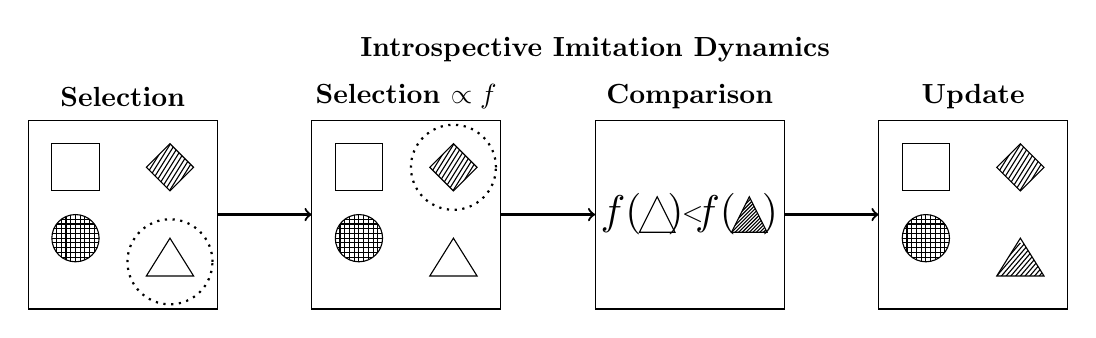
\begin{tikzpicture}[scale=0.6]

%================ FIRST BOX ==================
\draw (0,0) rectangle (4,4);

\draw (0.5,3.5) rectangle (1.5,2.5);

% Stripey diamond (sparser)
\begin{scope}
  \clip (2.5,3) -- (3,3.5) -- (3.5,3) -- (3,2.5) -- cycle;
  \foreach \x in {2.0,2.1,...,4.0} {
    \draw (\x,2.2) -- (\x+1,3.8);
  }
\end{scope}
\draw (2.5,3) -- (3,3.5) -- (3.5,3) -- (3,2.5) -- cycle;

% Cross-hatched circle (sparser)
\begin{scope}
  \clip (1,1.5) circle (0.5);
  \foreach \x in {0.3,0.4,...,1.7} {
    \draw (\x,1) -- (\x,2);
  }
  \foreach \y in {1,1.1,...,2} {
    \draw (0.3,\y) -- (1.7,\y);
  }
\end{scope}
\draw (1,1.5) circle (0.5);

% Triangle (plain)
\draw (3,1.5) -- (2.5,0.7) -- (3.5,0.7) -- cycle;


%================ 2nd box (SHIFTED RIGHT) ==================
\draw (6,0) rectangle (10,4);
\node at (8,4.5) {\textbf{Selection \(\propto f\)}};

\draw (6.5,3.5) rectangle (7.5,2.5);

\begin{scope}
  \clip (8.5,3) -- (9,3.5) -- (9.5,3) -- (9,2.5) -- cycle;
  \foreach \x in {8.0,8.1,...,10.0} {
    \draw (\x,2.2) -- (\x+1,3.8);
  }
\end{scope}
\draw (8.5,3) -- (9,3.5) -- (9.5,3) -- (9,2.5) -- cycle;

\begin{scope}
  \clip (7,1.5) circle (0.5);
  \foreach \x in {6.3,6.4,...,7.7} {
    \draw (\x,1) -- (\x,2);
  }
  \foreach \y in {1,1.1,...,2} {
    \draw (6.3,\y) -- (7.7,\y);
  }
\end{scope}
\draw (7,1.5) circle (0.5);

\draw (9,1.5) -- (8.5,0.7) -- (9.5,0.7) -- cycle;

\draw[dotted, thick] (9,3) circle (0.9cm);


%================ 3rd box (SHIFTED RIGHT) ==================
\draw (12,0) rectangle (16,4);

\node[scale=1.5] at (12.55,2) {$f($};
\node[scale=1.5] at (14.55,2) {$f($};
\begin{scope}[shift={(13.2,2)}, scale=0.75]
    % --- plain (empty) triangle ---
    \draw (0.15,0.5) -- (-0.35,-0.5) -- (0.65,-0.5) -- cycle;

    % --- less-than symbol ---
    \node at (1.15,0) {$<$};

    % --- stripey black triangle ---
    \draw (2.75,0.5) -- (2.25,-0.5) -- (3.25,-0.5) -- cycle;

    \clip (2.75,0.5) -- (2.25,-0.5) -- (3.25,-0.5) -- cycle;
        \foreach \x in {-1.05,-0.95,...,3.25} {
            \draw (\x,-1) -- (\x+2,1);
        }
\end{scope}
\node[scale=1.5] at (13.7,2) {$)$};
\node[scale=1.5] at (15.7,2) {$)$};


%================ 4th box (SHIFTED RIGHT) ==================
\draw (18,0) rectangle (22,4);

\draw (18.5,3.5) rectangle (19.5,2.5);

\begin{scope}
  \clip (20.5,3) -- (21,3.5) -- (21.5,3) -- (21,2.5) -- cycle;
  \foreach \x in {20.0,20.1,...,22.0} {
    \draw (\x,2.2) -- (\x+1,3.8);
  }
\end{scope}
\draw (20.5,3) -- (21,3.5) -- (21.5,3) -- (21,2.5) -- cycle;

\begin{scope}
  \clip (19,1.5) circle (0.5);
  \foreach \x in {18.3,18.4,...,19.7} {
    \draw (\x,1) -- (\x,2);
  }
  \foreach \y in {1,1.1,...,2} {
    \draw (18.3,\y) -- (19.7,\y);
  }
\end{scope}
\draw (19,1.5) circle (0.5);

\begin{scope}
  \clip (21,1.5) -- (20.5,0.7) -- (21.5,0.7) -- cycle;
  \foreach \x in {18.5,18.6,...,22} {
    \draw (\x,0.0) -- (\x+1.2,1.4);
  }
\end{scope}
\draw (21,1.5) -- (20.5,0.7) -- (21.5,0.7) -- cycle;


%================ ARROWS (SHIFTED RIGHT) ==================
\draw[->, thick] (4,2) -- (6,2);    
\draw[->, thick] (10,2) -- (12,2);   
\draw[->, thick] (16,2) -- (18,2);   


%================ HEADERS ==================
\node at (2,4.5) {\textbf{Selection}};
\node at (12,5.5) {\textbf{Introspective Imitation Dynamics}};
\node at (14,4.5) {\textbf{Comparison}};
\node at (20,4.5) {\textbf{Update}};

\draw[dotted, thick] (3,1) circle (0.9cm);

\end{tikzpicture}
&
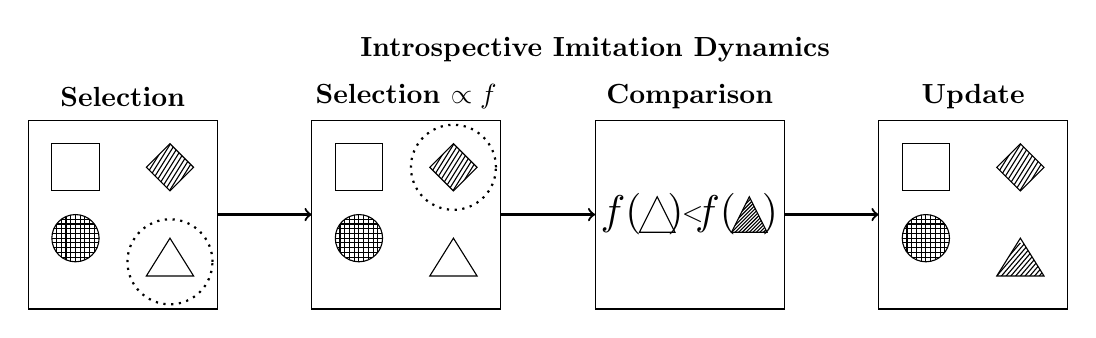
\begin{tikzpicture}[scale=0.6]

%================ FIRST BOX ==================
\draw (0,0) rectangle (4,4);

\draw (0.5,3.5) rectangle (1.5,2.5);

% Stripey diamond (sparser)
\begin{scope}
  \clip (2.5,3) -- (3,3.5) -- (3.5,3) -- (3,2.5) -- cycle;
  \foreach \x in {2.0,2.1,...,4.0} {
    \draw (\x,2.2) -- (\x+1,3.8);
  }
\end{scope}
\draw (2.5,3) -- (3,3.5) -- (3.5,3) -- (3,2.5) -- cycle;

% Cross-hatched circle (sparser)
\begin{scope}
  \clip (1,1.5) circle (0.5);
  \foreach \x in {0.3,0.4,...,1.7} {
    \draw (\x,1) -- (\x,2);
  }
  \foreach \y in {1,1.1,...,2} {
    \draw (0.3,\y) -- (1.7,\y);
  }
\end{scope}
\draw (1,1.5) circle (0.5);

% Triangle (plain)
\draw (3,1.5) -- (2.5,0.7) -- (3.5,0.7) -- cycle;


%================ 2nd box (SHIFTED RIGHT) ==================
\draw (6,0) rectangle (10,4);
\node at (8,4.5) {\textbf{Selection \(\propto f\)}};

\draw (6.5,3.5) rectangle (7.5,2.5);

\begin{scope}
  \clip (8.5,3) -- (9,3.5) -- (9.5,3) -- (9,2.5) -- cycle;
  \foreach \x in {8.0,8.1,...,10.0} {
    \draw (\x,2.2) -- (\x+1,3.8);
  }
\end{scope}
\draw (8.5,3) -- (9,3.5) -- (9.5,3) -- (9,2.5) -- cycle;

\begin{scope}
  \clip (7,1.5) circle (0.5);
  \foreach \x in {6.3,6.4,...,7.7} {
    \draw (\x,1) -- (\x,2);
  }
  \foreach \y in {1,1.1,...,2} {
    \draw (6.3,\y) -- (7.7,\y);
  }
\end{scope}
\draw (7,1.5) circle (0.5);

\draw (9,1.5) -- (8.5,0.7) -- (9.5,0.7) -- cycle;

\draw[dotted, thick] (9,3) circle (0.9cm);


%================ 3rd box (SHIFTED RIGHT) ==================
\draw (12,0) rectangle (16,4);

\node[scale=1.5] at (12.55,2) {$f($};
\node[scale=1.5] at (14.55,2) {$f($};
\begin{scope}[shift={(13.2,2)}, scale=0.75]
    % --- plain (empty) triangle ---
    \draw (0.15,0.5) -- (-0.35,-0.5) -- (0.65,-0.5) -- cycle;

    % --- less-than symbol ---
    \node at (1.15,0) {$<$};

    % --- stripey black triangle ---
    \draw (2.75,0.5) -- (2.25,-0.5) -- (3.25,-0.5) -- cycle;

    \clip (2.75,0.5) -- (2.25,-0.5) -- (3.25,-0.5) -- cycle;
        \foreach \x in {-1.05,-0.95,...,3.25} {
            \draw (\x,-1) -- (\x+2,1);
        }
\end{scope}
\node[scale=1.5] at (13.7,2) {$)$};
\node[scale=1.5] at (15.7,2) {$)$};


%================ 4th box (SHIFTED RIGHT) ==================
\draw (18,0) rectangle (22,4);

\draw (18.5,3.5) rectangle (19.5,2.5);

\begin{scope}
  \clip (20.5,3) -- (21,3.5) -- (21.5,3) -- (21,2.5) -- cycle;
  \foreach \x in {20.0,20.1,...,22.0} {
    \draw (\x,2.2) -- (\x+1,3.8);
  }
\end{scope}
\draw (20.5,3) -- (21,3.5) -- (21.5,3) -- (21,2.5) -- cycle;

\begin{scope}
  \clip (19,1.5) circle (0.5);
  \foreach \x in {18.3,18.4,...,19.7} {
    \draw (\x,1) -- (\x,2);
  }
  \foreach \y in {1,1.1,...,2} {
    \draw (18.3,\y) -- (19.7,\y);
  }
\end{scope}
\draw (19,1.5) circle (0.5);

\begin{scope}
  \clip (21,1.5) -- (20.5,0.7) -- (21.5,0.7) -- cycle;
  \foreach \x in {18.5,18.6,...,22} {
    \draw (\x,0.0) -- (\x+1.2,1.4);
  }
\end{scope}
\draw (21,1.5) -- (20.5,0.7) -- (21.5,0.7) -- cycle;


%================ ARROWS (SHIFTED RIGHT) ==================
\draw[->, thick] (4,2) -- (6,2);    
\draw[->, thick] (10,2) -- (12,2);   
\draw[->, thick] (16,2) -- (18,2);   


%================ HEADERS ==================
\node at (2,4.5) {\textbf{Selection}};
\node at (12,5.5) {\textbf{Introspective Imitation Dynamics}};
\node at (14,4.5) {\textbf{Comparison}};
\node at (20,4.5) {\textbf{Update}};

\draw[dotted, thick] (3,1) circle (0.9cm);

\end{tikzpicture}
\\
&\\
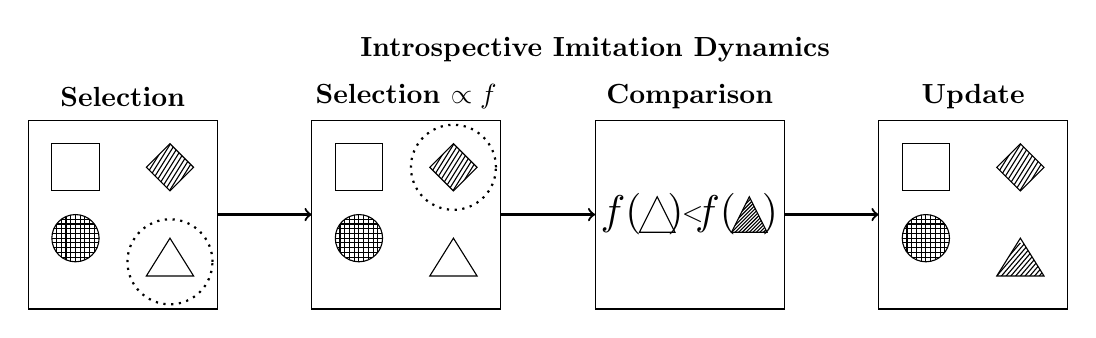
\begin{tikzpicture}[scale=0.6]

%================ FIRST BOX ==================
\draw (0,0) rectangle (4,4);

\draw (0.5,3.5) rectangle (1.5,2.5);

% Stripey diamond (sparser)
\begin{scope}
  \clip (2.5,3) -- (3,3.5) -- (3.5,3) -- (3,2.5) -- cycle;
  \foreach \x in {2.0,2.1,...,4.0} {
    \draw (\x,2.2) -- (\x+1,3.8);
  }
\end{scope}
\draw (2.5,3) -- (3,3.5) -- (3.5,3) -- (3,2.5) -- cycle;

% Cross-hatched circle (sparser)
\begin{scope}
  \clip (1,1.5) circle (0.5);
  \foreach \x in {0.3,0.4,...,1.7} {
    \draw (\x,1) -- (\x,2);
  }
  \foreach \y in {1,1.1,...,2} {
    \draw (0.3,\y) -- (1.7,\y);
  }
\end{scope}
\draw (1,1.5) circle (0.5);

% Triangle (plain)
\draw (3,1.5) -- (2.5,0.7) -- (3.5,0.7) -- cycle;


%================ 2nd box (SHIFTED RIGHT) ==================
\draw (6,0) rectangle (10,4);
\node at (8,4.5) {\textbf{Selection \(\propto f\)}};

\draw (6.5,3.5) rectangle (7.5,2.5);

\begin{scope}
  \clip (8.5,3) -- (9,3.5) -- (9.5,3) -- (9,2.5) -- cycle;
  \foreach \x in {8.0,8.1,...,10.0} {
    \draw (\x,2.2) -- (\x+1,3.8);
  }
\end{scope}
\draw (8.5,3) -- (9,3.5) -- (9.5,3) -- (9,2.5) -- cycle;

\begin{scope}
  \clip (7,1.5) circle (0.5);
  \foreach \x in {6.3,6.4,...,7.7} {
    \draw (\x,1) -- (\x,2);
  }
  \foreach \y in {1,1.1,...,2} {
    \draw (6.3,\y) -- (7.7,\y);
  }
\end{scope}
\draw (7,1.5) circle (0.5);

\draw (9,1.5) -- (8.5,0.7) -- (9.5,0.7) -- cycle;

\draw[dotted, thick] (9,3) circle (0.9cm);


%================ 3rd box (SHIFTED RIGHT) ==================
\draw (12,0) rectangle (16,4);

\node[scale=1.5] at (12.55,2) {$f($};
\node[scale=1.5] at (14.55,2) {$f($};
\begin{scope}[shift={(13.2,2)}, scale=0.75]
    % --- plain (empty) triangle ---
    \draw (0.15,0.5) -- (-0.35,-0.5) -- (0.65,-0.5) -- cycle;

    % --- less-than symbol ---
    \node at (1.15,0) {$<$};

    % --- stripey black triangle ---
    \draw (2.75,0.5) -- (2.25,-0.5) -- (3.25,-0.5) -- cycle;

    \clip (2.75,0.5) -- (2.25,-0.5) -- (3.25,-0.5) -- cycle;
        \foreach \x in {-1.05,-0.95,...,3.25} {
            \draw (\x,-1) -- (\x+2,1);
        }
\end{scope}
\node[scale=1.5] at (13.7,2) {$)$};
\node[scale=1.5] at (15.7,2) {$)$};


%================ 4th box (SHIFTED RIGHT) ==================
\draw (18,0) rectangle (22,4);

\draw (18.5,3.5) rectangle (19.5,2.5);

\begin{scope}
  \clip (20.5,3) -- (21,3.5) -- (21.5,3) -- (21,2.5) -- cycle;
  \foreach \x in {20.0,20.1,...,22.0} {
    \draw (\x,2.2) -- (\x+1,3.8);
  }
\end{scope}
\draw (20.5,3) -- (21,3.5) -- (21.5,3) -- (21,2.5) -- cycle;

\begin{scope}
  \clip (19,1.5) circle (0.5);
  \foreach \x in {18.3,18.4,...,19.7} {
    \draw (\x,1) -- (\x,2);
  }
  \foreach \y in {1,1.1,...,2} {
    \draw (18.3,\y) -- (19.7,\y);
  }
\end{scope}
\draw (19,1.5) circle (0.5);

\begin{scope}
  \clip (21,1.5) -- (20.5,0.7) -- (21.5,0.7) -- cycle;
  \foreach \x in {18.5,18.6,...,22} {
    \draw (\x,0.0) -- (\x+1.2,1.4);
  }
\end{scope}
\draw (21,1.5) -- (20.5,0.7) -- (21.5,0.7) -- cycle;


%================ ARROWS (SHIFTED RIGHT) ==================
\draw[->, thick] (4,2) -- (6,2);    
\draw[->, thick] (10,2) -- (12,2);   
\draw[->, thick] (16,2) -- (18,2);   


%================ HEADERS ==================
\node at (2,4.5) {\textbf{Selection}};
\node at (12,5.5) {\textbf{Introspective Imitation Dynamics}};
\node at (14,4.5) {\textbf{Comparison}};
\node at (20,4.5) {\textbf{Update}};

\draw[dotted, thick] (3,1) circle (0.9cm);

\end{tikzpicture}
&\\
&
\\
\hline
\multicolumn{2}{|c|}{Both Extrinsic and Intrinsic Strategy Analysis}\\
\hline
\multicolumn{2}{|c|}{ 
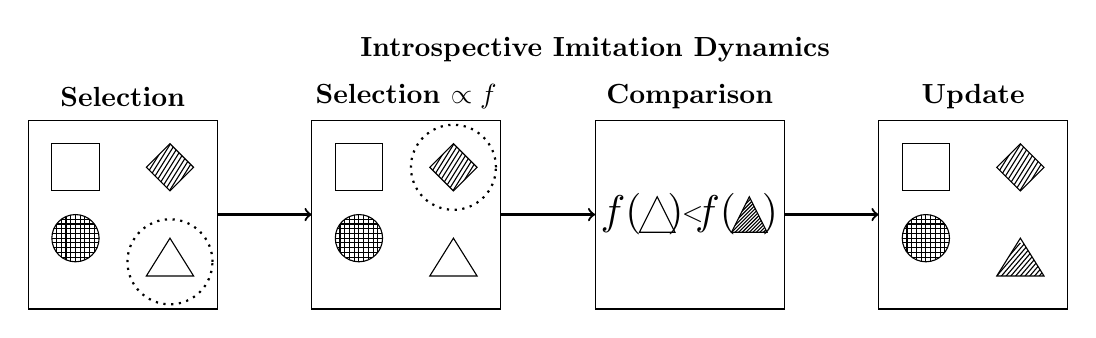
\begin{tikzpicture}[scale=0.6]

%================ FIRST BOX ==================
\draw (0,0) rectangle (4,4);

\draw (0.5,3.5) rectangle (1.5,2.5);

% Stripey diamond (sparser)
\begin{scope}
  \clip (2.5,3) -- (3,3.5) -- (3.5,3) -- (3,2.5) -- cycle;
  \foreach \x in {2.0,2.1,...,4.0} {
    \draw (\x,2.2) -- (\x+1,3.8);
  }
\end{scope}
\draw (2.5,3) -- (3,3.5) -- (3.5,3) -- (3,2.5) -- cycle;

% Cross-hatched circle (sparser)
\begin{scope}
  \clip (1,1.5) circle (0.5);
  \foreach \x in {0.3,0.4,...,1.7} {
    \draw (\x,1) -- (\x,2);
  }
  \foreach \y in {1,1.1,...,2} {
    \draw (0.3,\y) -- (1.7,\y);
  }
\end{scope}
\draw (1,1.5) circle (0.5);

% Triangle (plain)
\draw (3,1.5) -- (2.5,0.7) -- (3.5,0.7) -- cycle;


%================ 2nd box (SHIFTED RIGHT) ==================
\draw (6,0) rectangle (10,4);
\node at (8,4.5) {\textbf{Selection \(\propto f\)}};

\draw (6.5,3.5) rectangle (7.5,2.5);

\begin{scope}
  \clip (8.5,3) -- (9,3.5) -- (9.5,3) -- (9,2.5) -- cycle;
  \foreach \x in {8.0,8.1,...,10.0} {
    \draw (\x,2.2) -- (\x+1,3.8);
  }
\end{scope}
\draw (8.5,3) -- (9,3.5) -- (9.5,3) -- (9,2.5) -- cycle;

\begin{scope}
  \clip (7,1.5) circle (0.5);
  \foreach \x in {6.3,6.4,...,7.7} {
    \draw (\x,1) -- (\x,2);
  }
  \foreach \y in {1,1.1,...,2} {
    \draw (6.3,\y) -- (7.7,\y);
  }
\end{scope}
\draw (7,1.5) circle (0.5);

\draw (9,1.5) -- (8.5,0.7) -- (9.5,0.7) -- cycle;

\draw[dotted, thick] (9,3) circle (0.9cm);


%================ 3rd box (SHIFTED RIGHT) ==================
\draw (12,0) rectangle (16,4);

\node[scale=1.5] at (12.55,2) {$f($};
\node[scale=1.5] at (14.55,2) {$f($};
\begin{scope}[shift={(13.2,2)}, scale=0.75]
    % --- plain (empty) triangle ---
    \draw (0.15,0.5) -- (-0.35,-0.5) -- (0.65,-0.5) -- cycle;

    % --- less-than symbol ---
    \node at (1.15,0) {$<$};

    % --- stripey black triangle ---
    \draw (2.75,0.5) -- (2.25,-0.5) -- (3.25,-0.5) -- cycle;

    \clip (2.75,0.5) -- (2.25,-0.5) -- (3.25,-0.5) -- cycle;
        \foreach \x in {-1.05,-0.95,...,3.25} {
            \draw (\x,-1) -- (\x+2,1);
        }
\end{scope}
\node[scale=1.5] at (13.7,2) {$)$};
\node[scale=1.5] at (15.7,2) {$)$};


%================ 4th box (SHIFTED RIGHT) ==================
\draw (18,0) rectangle (22,4);

\draw (18.5,3.5) rectangle (19.5,2.5);

\begin{scope}
  \clip (20.5,3) -- (21,3.5) -- (21.5,3) -- (21,2.5) -- cycle;
  \foreach \x in {20.0,20.1,...,22.0} {
    \draw (\x,2.2) -- (\x+1,3.8);
  }
\end{scope}
\draw (20.5,3) -- (21,3.5) -- (21.5,3) -- (21,2.5) -- cycle;

\begin{scope}
  \clip (19,1.5) circle (0.5);
  \foreach \x in {18.3,18.4,...,19.7} {
    \draw (\x,1) -- (\x,2);
  }
  \foreach \y in {1,1.1,...,2} {
    \draw (18.3,\y) -- (19.7,\y);
  }
\end{scope}
\draw (19,1.5) circle (0.5);

\begin{scope}
  \clip (21,1.5) -- (20.5,0.7) -- (21.5,0.7) -- cycle;
  \foreach \x in {18.5,18.6,...,22} {
    \draw (\x,0.0) -- (\x+1.2,1.4);
  }
\end{scope}
\draw (21,1.5) -- (20.5,0.7) -- (21.5,0.7) -- cycle;


%================ ARROWS (SHIFTED RIGHT) ==================
\draw[->, thick] (4,2) -- (6,2);    
\draw[->, thick] (10,2) -- (12,2);   
\draw[->, thick] (16,2) -- (18,2);   


%================ HEADERS ==================
\node at (2,4.5) {\textbf{Selection}};
\node at (12,5.5) {\textbf{Introspective Imitation Dynamics}};
\node at (14,4.5) {\textbf{Comparison}};
\node at (20,4.5) {\textbf{Update}};

\draw[dotted, thick] (3,1) circle (0.9cm);

\end{tikzpicture}
}\\
\hline
\end{tabular}
\caption{A comparison of different population dynamics. We assume in all cases that the triangle is chosen for replacement with a probability \(\frac{1}{N}\) and the diamond is chosen with a varying probability depending on the process. In the case of Introspection dynamics, we assume that the strategy represented by the shape being filled in is chosen with probability \(\frac{1}{k-1}\)}
\end{table}



\section{The Public Goods Game}

\subsection{The Standard Model and Transformations}

In this section, we shall see how different population dynamics can be applied
to the public goods game. \cite{2bbcfd92-fcd5-38d1-b7a0-bc6a2aadbc64, hofbauer_sigmund_1998}
In this game, individuals choose whether or not to contribute to a public resource pool. 
In the end, the total resource is multiplied by some factor \(r > 1\) and distributed equally between each player. This model often encourages a behaviour known as ``free-riding" \cite{10.1257/aer.15000001}, where players refuse to contribute to the pool and simply take the benefit provided by other individuals' contribution. 
The classic problem of a public goods game is to provide an environment where such free-riding is less profitable than contributing to the public good.\\

We can model a public goods game by providing the following payoff function:\\
\begin{large}
\begin{equation}
    \pi_i(\textbf{a}) = \frac{r\sum_{j=1}^N{\alpha_j}}{N} - \alpha_i
    \label{eqn:General Model}
\end{equation}
\end{large}\\
(where \(\alpha_j\) is the contribution by individual j.) 
In the homogeneous public goods game, we have that \(\alpha_j\) can only take one of two values: some constant \(\alpha\) if individual j cooperates, and 0 if not. However, the heterogeneous game will require a more tailored \(\alpha_j\).\\

Note that \(\pi(v_j)\) can be negative, and such cannot be used as our fitness function for the Moran process. Therefore, we must look at some transformation of \(\pi\) to use as our fitness function.\\

A common method \cite{568a8a9c-d8ae-3d24-9fc2-3d33340230e7} for this is to apply the exponential function to our payoff function. By using \(e^{\beta \sigma}\) as our fitness function we will have positive values, however this particular approach gives, in the case of the Moran process:

\begin{large}
    \begin{equation}
        \frac{\sum_{a_i = b_{I(\textbf{a,b})}}{e^{\frac{\beta r\sum_{j=1}^N{\alpha_j}}{N} - \alpha_i}}}{\sum_{a_i}e^{\frac{\beta r\sum_{j=1}^N{\alpha_j}}{N} - \alpha_i}}
    \end{equation}
\end{large}\\

Now, as \(e^r\) does not rely on \(v\), we can take this out of the sum and acquire the following:

\begin{large}
    \begin{equation}
        \frac{e^{\frac{\beta r\sum_{j=1}^N{\alpha_j}}{N}}\sum_{a_i = b_{I(\textbf{a,b})}}{e^{ - \alpha_i}}}{e^{\frac{\beta r\sum_{j=1}^N{\alpha_j}}{N}}\sum_{a_i}e^{-C_{v_i}}} = \frac{\sum_{a_i = b_{I(\textbf{a,b})}}{e^{ - \alpha_i}}}{\sum_{a_i}e^{-\alpha_i}}
    \end{equation}
\end{large}\\

and we see that in this case, \(p_{a_j\to b_j}(a_{-j})\) would not rely on \(r\). 
Therefore, let us consider some other methods of guaranteeing a positive fitness function.\\

The first of these is known as the "shifted linear" transformation. We take, for some small tunable \(\epsilon\):
\begin{large}
    \begin{equation}
        f_i(\textbf{a}) = \pi_i(\textbf{a}) - \min_{j} \pi_j(\textbf{a}) + \beta
    \end{equation}
    \label{eqn:Shifted_linear}
\end{large}
This guarantees a positive value, with the lowest fitness taking the value \(\epsilon\), a parameter that can be chosen based on the system in question.
However, in the homogeneous case, as we can see in appendix[?], this mapping creates a fitness function which does not rely on \(r\), and so we cannot use this method.\\

%TODO - make appendix with the following:
%\begin{large}
%    \begin{equation}
%        \begin{split}
%        (\kappa_c(\textbf{a})r-\delta_j)\alpha - \min_j((\kappa_c(\textbf{a})r-\delta_j)\alpha)\alpha + \epsilon 
%        = (1 - \delta_i)\alpha + \epsilon = \begin{cases}
%            \epsilon & \text{if \(a_i\) contributes}\\
%            \alpha + \epsilon & \text{if not}
%        \end{cases}
%        \end{split}
%    \end{equation}
%    \label{eqn:Homogeneous_fitness}
%\end{large}\\


Another type of mapping that we can use is the ``Affine-linear mapping". In
this, for some tunable \(\epsilon\), we take the following:

\begin{large}
    \begin{equation}
        f_i(\textbf{a}) = 1 + \epsilon\pi_i(\textbf{a})
    \end{equation}
    \label{eqn:Affine-linear}
\end{large}\\
As \(\epsilon\) is a selection intensity parameter, this method both provides us a strictly positive fitness function for a well defined \(\epsilon\), and also allows us to control the selection intensity of the Moran process. 
Unlike in other population dynamics, this is not already defined within the Moran process, and so this is another benefit of using the affine-linear mapping.
Thus, we take this mapping of \(\pi\) as our fitness function.\\
In order to avoid having two selection intensity parameters, we can define \(\beta=1\) in this case, and allow \(\epsilon = \frac{1}{\beta}\), in order that we have \(\pi_i = 1 + \frac{f_i}{\beta}\).
Thus in the Fermi function we preserve the power of \(e^{\frac{\Delta(f)}{\beta}}\) for some selection intensity \(\beta\).
However, we will now have a bound on \(\beta\) depending on the values of \(\alpha\) in our public goods game, as we must define a strictly positive fitness function.


\subsection{The Homogeneous Case}
The most simple type of public goods game is the homogeneous public goods game.\cite{2bbcfd92-fcd5-38d1-b7a0-bc6a2aadbc64}
In this game, we consider that we have a constant \(\alpha_i = \alpha\) for all players \(a_i\).
In this case, we take the payoff function:
\begin{large}
    \begin{equation}
        \sigma(v_i) = \frac{r\sum_{j=1}^N{\delta_j\alpha}}{N} - \delta_j\alpha = (\kappa_c(\textbf{a})r-\delta_j)\alpha
    \end{equation}
    \label{eqn:Homogeneous_fitness}
\end{large}\\
Where \(\delta_j = 1\) if j contributes and 0 if not, and \(\kappa_c(\textbf{a})\) is the fraction of the population who contribute.\\

We will begin by looking at the state space with \(N=4\) and see how cooperation emerges based on different values of \(r \text{ and } \alpha\).

We can assign the value 0 to non-contribution and 1 contribution in the state space \(\textbf{a},\textbf{b},\textbf{c},\textbf{d}\),  and in doing so obtain the following absorption matrices for each population dynamic:\\

\begin{table}[!h]
    \centering
    \Large
        \begin{tabular}{|c|c|}
        \hline
        Moran Process & Introspection Dynamics \\
        \hline
        $\displaystyle
        \left[\begin{matrix}
        \frac{\alpha \epsilon r + 2}{\alpha \epsilon r + \alpha \epsilon (r - 2) + 4} &
        \frac{\alpha \epsilon (r - 2) + 2}{\alpha \epsilon r + \alpha \epsilon (r - 2) + 4} \\
        \frac{\alpha \epsilon r + 2}{\alpha \epsilon r + \alpha \epsilon (r - 2) + 4} &
        \frac{\alpha \epsilon (r - 2) + 2}{\alpha \epsilon r + \alpha \epsilon (r - 2) + 4}
        \end{matrix}\right]$
        &
        \tiny
        $\begin{bmatrix}
        \frac{1}{e^{\frac{\alpha \epsilon (r - 2)}{2 \beta}} + 1} & \frac{e^{\frac{\alpha \epsilon (r - 2)}{2 \beta}}}{2 \left(e^{\frac{\alpha \epsilon (r - 2)}{2 \beta}} + 1\right)} & \frac{e^{\frac{\alpha \epsilon (r - 2)}{2 \beta}}}{2 \left(e^{\frac{\alpha \epsilon (r - 2)}{2 \beta}} + 1\right)} & 0 \\
        \frac{1}{2 \left(e^{\frac{\alpha \epsilon (r - 2)}{2 \beta}} + 1\right)} & \frac{1}{2} & 0 & \frac{1}{2 \left(e^{\frac{\alpha \epsilon (2 - r)}{2 \beta}} + 1\right)} \\
        \frac{1}{2 \left(e^{\frac{\alpha \epsilon (r - 2)}{2 \beta}} + 1\right)} & 0 & \frac{1}{2} & \frac{1}{2 \left(e^{\frac{\alpha \epsilon (2 - r)}{2 \beta}} + 1\right)} \\
        0 & \frac{1}{2 \left(e^{\frac{\alpha \epsilon (r - 2)}{2 \beta}} + 1\right)} & \frac{1}{2 \left(e^{\frac{\alpha \epsilon (r - 2)}{2 \beta}} + 1\right)} & \frac{e^{\frac{\alpha \epsilon (r - 2)}{2 \beta}}}{e^{\frac{\alpha \epsilon (r - 2)}{2 \beta}} + 1}
        \end{bmatrix}
        $\\
         \hline
         Fermi Imitation Dynamics & Introspective Imitation Dynamics\\
         \hline
         $\displaystyle \left[\begin{matrix}\frac{ e^{\frac{\alpha}{\beta}}}{e^{\frac{\alpha}{\beta}} + 1} & \frac{1}{e^{\frac{\alpha}{\beta}} + 1}\\\frac{ e^{\frac{\alpha}{\beta}}}{e^{\frac{\alpha}{\beta}} + 1} & \frac{1}{e^{\frac{\alpha}{\beta}} + 1}\end{matrix}\right]$
         & \tiny
         $\displaystyle \left[\begin{matrix}\frac{\left(\alpha \epsilon r + 2\right) \left(e^{\frac{\alpha \epsilon \left(2 - r\right)}{2 \beta}} + 1\right)}{\left(\alpha \epsilon r + 2\right) \left(e^{\frac{\alpha \epsilon \left(2 - r\right)}{2 \beta}} + 1\right) + \left(\alpha \epsilon \left(r - 2\right) + 2\right) \left(e^{\frac{\alpha \epsilon \left(r - 2\right)}{2 \beta}} + 1\right)} & \frac{\left(\alpha \epsilon \left(r - 2\right) + 2\right) \left(e^{\frac{\alpha \epsilon \left(r - 2\right)}{2 \beta}} + 1\right)}{\left(\alpha \epsilon r + 2\right) \left(e^{\frac{\alpha \epsilon \left(2 - r\right)}{2 \beta}} + 1\right) + \left(\alpha \epsilon \left(r - 2\right) + 2\right) \left(e^{\frac{\alpha \epsilon \left(r - 2\right)}{2 \beta}} + 1\right)}\\\frac{\left(\alpha \epsilon r + 2\right) \left(e^{\frac{\alpha \epsilon \left(2 - r\right)}{2 \beta}} + 1\right)}{\left(\alpha \epsilon r + 2\right) \left(e^{\frac{\alpha \epsilon \left(2 - r\right)}{2 \beta}} + 1\right) + \left(\alpha \epsilon \left(r - 2\right) + 2\right) \left(e^{\frac{\alpha \epsilon \left(r - 2\right)}{2 \beta}} + 1\right)} & \frac{\left(\alpha \epsilon \left(r - 2\right) + 2\right) \left(e^{\frac{\alpha \epsilon \left(r - 2\right)}{2 \beta}} + 1\right)}{\left(\alpha \epsilon r + 2\right) \left(e^{\frac{\alpha \epsilon \left(2 - r\right)}{2 \beta}} + 1\right) + \left(\alpha \epsilon \left(r - 2\right) + 2\right) \left(e^{\frac{\alpha \epsilon \left(r - 2\right)}{2 \beta}} + 1\right)}\end{matrix}\right]$\\
         &\\
         \hline
    \end{tabular}
    \caption{A table of absorption probabilities for different population dynamics in the homogeneous public goods game. The row correspond to which state \textbf{b} or \textbf{c} we begin in, and the column corresponds to which state \textbf{a} or \textbf{d} we are absorbed into. Thus the right hand row is the absorption probability for full contribution, and the left hand row is the absorption probability for no contribution.}
    \label{tab:placeholder}
\end{table}


We see that in the homogeneous case of the 2 player public goods game, the absorption probabilities do not depend on which transitive state you begin in.
This is clear, as the states \(\textbf{b} = (0,1)\) and \(\textbf{c} = (1,0)\)
are equivalent due to there being no difference between players 1 and 2.

\subsection{Numerical Results}

We can now see how the different population dynamics affect the absorption
probabilities in the homogeneous public goods game. We first consider the
effect of r on our population in various \(\alpha\) values:

\begin{figure}[!h]
\centering

\includegraphics[width=0.8\textwidth]{../src/img/absorption_probabilities_vary_r_fix_alpha/main.pdf}
\hfill

\caption{The absorption probability of the homogeneous public goods game for varying \(r\) at different values of \(\alpha\)}
\end{figure}

The main point of interest here is the comparison betwee the Moran process and
introspective imitation dynamics.
We see that in the case of \(N=2\), the Moran process has a higher
absorption probability than introspective imitation dynamics for \(r<N\),
however it has a lower probability for \(r>N\).
Now, consider the fact that for \(r>N\), one should always contribute if acting
rationally, due to the fact that even by contributing themself, they will
always make a profit. 
Conversely, for \(r<1\), one should never contribute in any population, as even
with all players contributing, all make a loss.
Thus, the most realistic population dynamic is that which has the highest
absorption probability for \(r>N\), and also the lowest absorption probability
for \(r<1\). 
When compared to the Moran process, we have that these considerations favour
introspective imitation dynamics.

Now let us consider the impact of different selection intensities on the
absorption probability of these dynamics.




\newpage
\section{Public Goods Games with Heterogeneous Returns}

When we look at a public goods game, we often generalise the players to all receive the same return. However, in the real world this is often not the case. 


\bibliographystyle{plain}
\bibliography{bibliography.bib}
\end{document}